\documentclass[11pt,a4paper]{article}

% ── Packages ──────────────────────────────────────────────────────────
\usepackage[utf8]{inputenc}
\usepackage[T1]{fontenc}
\usepackage{amsmath,amssymb,amsthm}
\usepackage{algorithm}
\usepackage[noend]{algpseudocode}
\usepackage{graphicx}
\usepackage{booktabs}
\usepackage{multirow}
\usepackage{xcolor}
\usepackage{hyperref}
\usepackage[margin=2.5cm]{geometry}
\usepackage{subcaption}
\usepackage{enumitem}
\usepackage{cleveref}

% ── Colours ───────────────────────────────────────────────────────────
\definecolor{improved}{HTML}{2ca02c}
\definecolor{baseline}{HTML}{7f7f7f}

% ── Algorithmic customisation ─────────────────────────────────────────
\algnewcommand\algorithmicforeach{\textbf{for each}}
\algdef{S}[FOR]{ForEach}[1]{\algorithmicforeach\ #1\ \algorithmicdo}
\algnewcommand\algorithmicinput{\textbf{Input:}}
\algnewcommand\algorithmicoutput{\textbf{Output:}}
\algnewcommand\Input{\item[\algorithmicinput]}
\algnewcommand\Output{\item[\algorithmicoutput]}

% ── Math macros ───────────────────────────────────────────────────────
\newcommand{\calP}{\mathcal{P}}
\newcommand{\calA}{\mathcal{A}}
\newcommand{\calN}{\mathcal{N}}
\newcommand{\calS}{\mathcal{S}}
\newcommand{\calF}{\mathcal{F}}
\newcommand{\calI}{\mathcal{I}}
\newcommand{\bbR}{\mathbb{R}}
\DeclareMathOperator*{\argmin}{arg\,min}
\DeclareMathOperator*{\argmax}{arg\,max}

% ══════════════════════════════════════════════════════════════════════
\title{%
  Enhanced Pareto Local Search for the\\
  Satellite Image Mosaic Selection Problem:\\
  Greedy Initialisation, Checkpoint-Based Tracking,\\
  and Perturbation Restart%
}
\author{%
  Anonymous Authors%
}
\date{}

\begin{document}
\maketitle

% ══════════════════════════════════════════════════════════════════════
\begin{abstract}
The Satellite Image Mosaic Selection (SIMS) problem requires choosing a
cost-effective set of satellite images that jointly cover a geographic area
of interest while simultaneously minimising acquisition cost, cloud
coverage, spatial resolution loss, and worst-case incidence angle.  We
present three complementary enhancements to the Pareto Local Search (PLS)
heuristic that serves as the metaheuristic engine inside a hybrid
exact/heuristic solver framework.

First, we introduce a \emph{greedy multi-objective initialisation}
strategy that seeds the search with diverse, high-quality feasible
solutions constructed via weighted greedy set cover using
$\binom{D}{1}+\binom{D}{2}+1$ weight vectors, where $D$ is the number of
objectives.  Second, we propose a \emph{two-level checkpoint mechanism}
for the incremental objective trackers that replaces repeated per-image
undo operations with bulk state restoration, yielding constant-time
state transitions during neighbourhood evaluation.  Third, we design a
\emph{perturbation-based restart} that, when the $k{=}1$ neighbourhood is
exhausted, injects randomly perturbed archive solutions back into the
working population, providing diversification without the combinatorial
expense of higher-order neighbourhoods.

Experiments across 20 benchmark instances (5~cities $\times$ 4~sizes,
30--150~images, 4~objectives) show that the combined enhancements
improve normalised hypervolume by up to $+57.8\%$ and by $+11.7\%$ on
average over the baseline PLS, with the largest gains on instances where
the baseline converges prematurely.  Hypervolume-over-time curves confirm
that the improvements manifest within the first seconds of execution and
persist throughout the run.
\end{abstract}

\paragraph{Keywords.}
multi-objective optimisation, Pareto local search, satellite image
selection, set cover, hypervolume, greedy initialisation, perturbation
restart

% ══════════════════════════════════════════════════════════════════════
\section{Introduction}\label{sec:intro}

Earth observation planning increasingly relies on automated methods to
select mosaics of satellite images that cover a region of interest (ROI)
while balancing conflicting quality criteria.  The resulting
\emph{Satellite Image Mosaic Selection} (SIMS) problem is a
multi-objective variant of the weighted set cover problem and is known to
be NP-hard.

In a companion study we developed a \emph{two-phase hybrid} solver that
allocates part of the time budget to an exact method
(AUGMECON/GPBA-based MILP) and the remainder to a Pareto Local Search
(PLS) metaheuristic.  The exact phase produces a small set of provably
efficient anchor solutions; PLS then densifies the Pareto front around
and between them.  The quality of the final approximation set depends
critically on the effectiveness of PLS, which in turn depends on (i)~the
quality of its starting population, (ii)~the throughput of its
neighbourhood evaluation, and (iii)~its ability to escape local optima.

\paragraph{Contributions.}
We identify three independent weaknesses of the baseline PLS and propose
targeted fixes:

\begin{enumerate}[leftmargin=*,nosep]
  \item \textbf{Greedy multi-objective initialisation}
    (\Cref{sec:greedy}): replaces the random initial population with
    diverse feasible solutions constructed by a weighted greedy set-cover
    heuristic, one per objective axis, per objective pair, and one
    balanced, giving $\binom{D}{1}+\binom{D}{2}+1$ anchor points.
  \item \textbf{Two-level checkpoint mechanism} (\Cref{sec:checkpoint}):
    introduces $O(1)$ bulk state restore for incremental objective
    trackers, eliminating redundant per-image undo operations during
    neighbourhood enumeration.
  \item \textbf{Perturbation restart} (\Cref{sec:perturb}): when the
    working population's $k{=}1$ neighbourhood is exhausted, randomly
    perturbed copies of archive solutions are injected, resetting the
    neighbourhood level and avoiding the combinatorial cost of
    $k{\ge}2$.
\end{enumerate}

Each technique is independently toggleable, enabling controlled ablation.
We evaluate all combinations on 15~instances with $D{=}4$ objectives and
report hypervolume improvements of up to~$60\%$.

% ══════════════════════════════════════════════════════════════════════
\section{Problem Formulation}\label{sec:problem}

\subsection{Decision Space}

An instance of SIMS comprises a universe $U = \{1,\ldots,m\}$ of
geographic segments (elements), a catalogue $\calI = \{1,\ldots,n\}$ of
candidate satellite images, and for each image~$i$ the set $S_i
\subseteq U$ of elements it covers.  A \emph{feasible mosaic} is a
subset $X \subseteq \calI$ such that $\bigcup_{i \in X} S_i = U$, i.e.\
a \emph{set cover}.  Instance sizes in our benchmark range from
$n{=}30,\; m{=}298$ to $n{=}200,\; m{=}25\,271$.

\subsection{Objective Space}

All four objectives are to be \emph{minimised}:
\begin{align}
  f_1(X) &= \sum_{i \in X} c_i
    &&\text{(total acquisition cost),} \label{eq:cost}\\
  f_2(X) &= \sum_{e \in U} a_e \cdot
    \mathbf{1}\!\bigl[\,\forall\, i \in X:\; e \notin C_i\bigr]
    &&\text{(cloudy area),} \label{eq:cloud}\\
  f_3(X) &= \sum_{e \in U}
    \min_{i \in X:\, e \in S_i} r_i
    &&\text{(resolution sum),} \label{eq:res}\\
  f_4(X) &= \max_{i \in X}\; \alpha_i
    &&\text{(worst incidence angle),} \label{eq:angle}
\end{align}
where $c_i$ is the per-image cost, $a_e$ is the area of element~$e$,
$C_i \subseteq S_i$ denotes the \emph{clear} elements of image~$i$
(complement of cloud mask within coverage), $r_i$ is the spatial
resolution of image~$i$, and $\alpha_i$ its incidence angle.

\medskip\noindent
Objectives \eqref{eq:cost}--\eqref{eq:res} are \emph{additive or
element-wise aggregations} over the selected images, while
\eqref{eq:angle} is a \emph{bottleneck} (max) objective.  This
structural heterogeneity has important consequences for neighbourhood
design and incremental evaluation.

% ══════════════════════════════════════════════════════════════════════
\section{Baseline PLS}\label{sec:pls_baseline}

Our starting point is a population-based PLS with the classic
\emph{accept non-dominated neighbours} acceptance criterion and a
\emph{variable neighbourhood structure} $k \in \{1,\ldots,k_{\max}\}$.

\subsection{Neighbourhood Operator}\label{sec:neighbourhood}

The neighbourhood $\calN_k(X)$ of a feasible solution~$X$ is defined by
a \emph{remove-then-repair} scheme:

\begin{enumerate}[nosep]
  \item \textbf{Remove} $k$ selected images from~$X$, producing a
    partial solution $X' = X \setminus R$ with $|R|=k$.
  \item \textbf{Identify} uncovered elements
    $U' = U \setminus \bigcup_{i \in X'} S_i$.
  \item \textbf{Repair}: select a \emph{condensed} sub-problem of the
    $\ell$ best addition candidates (ranked by a random weighted
    scalarisation of objective deltas) and enumerate all subsets that
    restore coverage, yielding a set of feasible neighbours.
\end{enumerate}

For $k{=}1$, every selected image that is \emph{replaceable} (at least
one unselected image overlaps with it) is a removal candidate.  For
$k{>}1$, the algorithm selects the $q{=}9$ worst-scoring images and
iterates over $\binom{q}{k}$ removal combinations.

\subsection{Incremental Objective Trackers}\label{sec:trackers}

Evaluating objectives from scratch for each neighbour is prohibitively
expensive.  Instead, four \emph{incremental trackers} maintain mutable
state that is updated in $O(|S_i|)$ time per image addition or removal:

\begin{itemize}[nosep]
  \item \textbf{TotalCost:} a running scalar sum; $O(1)$ delta.
  \item \textbf{CloudyArea:} per-element counters
    $\texttt{clear\_count}[e]$; delta when counter transitions $0
    \leftrightarrow 1$.
  \item \textbf{MinResolution:} per-element packed level-count arrays
    tracking the minimum resolution among covering images;
    $O(|S_i|)$ delta per add/remove.
  \item \textbf{MaxIncidenceAngle:} sorted level-count array of
    selected-image angles; $O(L)$ delta where $L$ is the number of
    distinct angle values (typically ${\le}30$).
\end{itemize}

\subsection{Main Loop}

The PLS main loop (\Cref{alg:pls_baseline}) iterates as follows.  At
each \emph{step}, every solution in the current working population is
explored: its neighbourhood $\calN_k$ is enumerated, and non-dominated
neighbours that have not been seen before are added to both the global
Pareto archive~$\calA$ and an \emph{auxiliary population}.  If the
auxiliary population is non-empty, it replaces the working population and
$k$ resets to~$1$.  Otherwise $k$ is incremented; if $k > k_{\max}$ the
algorithm terminates.

\begin{algorithm}[t]
\caption{Baseline Pareto Local Search}\label{alg:pls_baseline}
\begin{algorithmic}[1]
\Input problem instance $(U,\calI,f_1,\ldots,f_D)$, timeout $T$, $k_{\max}$
\Output approximate Pareto set $\calA$

\State $P \gets$ random feasible solutions; \quad $\calA \gets P$; \quad $k \gets 1$
\While{elapsed time $< T$}
  \State $P_{\mathrm{aux}} \gets \emptyset$
  \ForEach{$X \in \textsc{Shuffle}(P)$}
    \ForEach{$X' \in \calN_k(X)$}
      \If{$X'$ not previously explored \textbf{and} $X'$ is non-dominated w.r.t.\ $\calA$}
        \State $\calA.\textsc{Insert}(X')$; \quad $P_{\mathrm{aux}}.\textsc{Insert}(X')$
      \EndIf
    \EndFor
  \EndFor
  \If{$P_{\mathrm{aux}} \neq \emptyset$}
    \State $P \gets P_{\mathrm{aux}}$; \quad $k \gets 1$  \Comment{restart with new population}
  \ElsIf{$k < k_{\max}$}
    \State $k \gets k + 1$; \quad add eligible archive solutions to $P$
  \Else
    \State \textbf{break} \Comment{all neighbourhood structures exhausted}
  \EndIf
\EndWhile
\State \Return $\calA$
\end{algorithmic}
\end{algorithm}

% ══════════════════════════════════════════════════════════════════════
\section{Enhancement 1: Greedy Multi-Objective Initialisation}
\label{sec:greedy}

\subsection{Motivation}

The baseline PLS generates its initial population by constructing 100
random feasible solutions.  Because the SIMS objective space is
four-dimensional and the set-cover constraint is non-trivial, random
solutions tend to cluster in a narrow region of the Pareto front,
leaving large portions of the objective space unexplored during early
iterations.  Metaheuristics such as NSGA-II and MOEA/D mitigate this
with population-diversity mechanisms (crowding distance, decomposition
vectors); PLS has no such mechanism by default.

\subsection{Method}

We construct a small set of diverse, high-quality feasible solutions
using a \emph{weighted greedy set-cover} heuristic
(\Cref{alg:greedy}).  The greedy heuristic accepts a weight vector
$\mathbf{w} \in \bbR^D_{\ge 0}$ and iteratively selects the image with
the best weighted score per newly covered element until coverage is
complete.

\begin{algorithm}[t]
\caption{Weighted Greedy Set-Cover Construction}\label{alg:greedy}
\begin{algorithmic}[1]
\Input problem instance, weight vector $\mathbf{w} \in \bbR^D$
\Output feasible solution $X$

\State Pre-compute per-image objective proxy values $v_i^{(d)}$ for
  each image $i$ and objective $d$:
  \Statex \quad $v_i^{(\text{cost})} = c_i$, \;
    $v_i^{(\text{cloud})} = |S_i \setminus C_i|$, \;
    $v_i^{(\text{res})} = r_i$, \;
    $v_i^{(\text{angle})} = \alpha_i$
\State $X \gets \emptyset$; \quad $\textit{covered} \gets \emptyset$
\While{$\textit{covered} \neq U$}
  \ForEach{unselected image $i \notin X$}
    \State $\delta_i \gets |\{e \in S_i : e \notin \textit{covered}\}|$
      \Comment{newly covered elements}
    \If{$\delta_i > 0$}
      \State $\textit{score}_i \gets
        \bigl(\sum_{d=1}^{D} w_d \cdot v_i^{(d)}\bigr) \,/\, \delta_i$
    \EndIf
  \EndFor
  \State $i^* \gets \argmin_{i:\,\delta_i>0} \textit{score}_i$
  \State $X \gets X \cup \{i^*\}$; \quad
    $\textit{covered} \gets \textit{covered} \cup S_{i^*}$
\EndWhile
\State \Return $X$
\end{algorithmic}
\end{algorithm}

To achieve broad coverage of the objective space, we invoke
\Cref{alg:greedy} with a structured set of weight vectors:

\begin{enumerate}[nosep]
  \item $D$ \textbf{axis-aligned} vectors $\mathbf{e}_d$ (weight~1 on
    objective~$d$, 0~elsewhere), each producing a solution that greedily
    minimises one objective;
  \item $\binom{D}{2}$ \textbf{pairwise} vectors with weight~$0.5$ on
    each of two objectives, covering trade-off regions between pairs;
  \item 1 \textbf{balanced} vector $\mathbf{w} = (\tfrac{1}{D},\ldots,
    \tfrac{1}{D})$.
\end{enumerate}

For $D{=}4$ this yields $4 + 6 + 1 = 11$ greedy solutions.  These are
inserted into the initial population alongside the 100 random solutions
and filtered through the Pareto archive, providing non-dominated anchor
points in diverse regions of the front from the very first iteration.

\subsection{Complexity}

Each greedy construction is $O(n \cdot m)$ (at most $n$ iterations, each
scanning $n$ images over $m$ elements).  With 11~invocations the total
initialisation overhead is $O(11 \cdot n \cdot m)$, negligible compared
to PLS exploration.

% ══════════════════════════════════════════════════════════════════════
\section{Enhancement 2: Two-Level Checkpoint Mechanism}
\label{sec:checkpoint}

\subsection{Motivation}

During neighbourhood evaluation, the baseline PLS modifies shared
tracker state following the remove-then-repair scheme.  For each removal
combination, the tracker transitions through the following states:
\[
  \underbrace{S_{\mathrm{base}}}_{\text{original}}
  \;\xrightarrow{\text{remove } k \text{ images}}\;
  \underbrace{S_{\mathrm{removed}}}_{\text{partial}}
  \;\xrightarrow[\text{for each residual}]{\text{add images}}\;
  S_{\mathrm{merged}}
  \;\xrightarrow{\text{undo}}\;
  S_{\mathrm{removed}}
  \;\xrightarrow{\text{restore}}\;
  S_{\mathrm{base}}
\]

In the baseline, each transition is performed by iterating over
individual images and calling \texttt{track\_image\_addition} or
\texttt{track\_image\_removal}, each costing $O(|S_i|)$ for the
CloudyArea and MinResolution trackers.  With hundreds of residual
solutions per removal combination and dozens of removal combinations per
solution, these undo operations dominate wall-clock time.

\subsection{Method}

We observe that the mutable tracker state can be captured and restored
as a compact snapshot.  This makes it possible to replace long sequences
of undo operations with direct restoration of previously saved states.
We introduce \emph{two checkpoint levels} (\Cref{fig:checkpoint}):

\begin{description}[nosep,leftmargin=1.5em]
  \item[Base checkpoint:] snapshot of the original tracker state before
    any removals.  It is used to restore the tracker when transitioning
    between different removal combinations.
  \item[Removed-state checkpoint:] snapshot of the tracker state after a
    particular set of $k$~image removals.  It is used to restore the
    tracker after evaluating each repaired neighbour, replacing repeated
    per-image undo operations.
\end{description}

\begin{figure}[t]
\centering
\small
\setlength{\fboxsep}{6pt}
\fbox{\parbox{0.92\linewidth}{%
\textbf{Baseline tracker transitions} (per removal combination):\\[4pt]
$\text{original state}
  \xrightarrow[\scriptstyle O(k \cdot |S_i|)]{\text{remove}}
  \text{post-removal state}
  \xrightarrow[\scriptstyle O(|S_j|)]{\text{repair}_1}
  \text{candidate state}_1
  \xrightarrow[\scriptstyle O(|S_j|)]{\text{undo}_1}
  \text{post-removal state}
  \xrightarrow[\scriptstyle O(|S_j|)]{\text{repair}_2}
  \text{candidate state}_2
  \xrightarrow[\scriptstyle O(|S_j|)]{\text{undo}_2}
  \text{post-removal state}
  \;\cdots
  \xrightarrow[\scriptstyle O(k \cdot |S_i|)]{\text{restore}}
  \text{original state}$
\\[8pt]
\textbf{Checkpoint tracker transitions:}\\[4pt]
$\underset{\scriptstyle\text{save base checkpoint}}{\boxed{\text{original state}}}
  \xrightarrow[\scriptstyle O(k \cdot |S_i|)]{\text{remove}}
  \underset{\scriptstyle\text{save removal checkpoint}}{\boxed{\text{post-removal state}}}
  \xrightarrow[\scriptstyle O(|S_j|)]{\text{repair}_1}
  \text{candidate state}_1
  \xrightarrow[\scriptstyle O(1)\;\text{restore}]{\text{removal checkpoint}}
  \text{post-removal state}
  \xrightarrow[\scriptstyle O(|S_j|)]{\text{repair}_2}
  \text{candidate state}_2
  \xrightarrow[\scriptstyle O(1)\;\text{restore}]{\text{removal checkpoint}}
  \text{post-removal state}
  \;\cdots
  \xrightarrow[\scriptstyle O(1)\;\text{restore}]{\text{base checkpoint}}
  \text{original state}$
}}
\caption{Tracker state transitions during neighbourhood evaluation.  The
  checkpoint mechanism replaces iterative per-image undo with direct
  restoration of previously saved tracker states.  The ``$O(1)$''
  annotation refers to fixed-size state restoration whose cost depends
  on the universe size~$m$ but is independent of the number of images
  involved.}
\label{fig:checkpoint}
\end{figure}

The checkpoint operation copies only the mutable portions of each
tracker, leaving immutable shared data in place.  In practice, the
resulting snapshots are small enough that restoration remains cheap
relative to repeated per-image undo operations, even on the larger
instances considered in our benchmark.

\subsection{Pseudocode}

\Cref{alg:checkpoint_iter} presents the enhanced neighbourhood
evaluation procedure.

\begin{algorithm}[t]
\caption{Neighbourhood Iterator with Two-Level Checkpointing}
\label{alg:checkpoint_iter}
\begin{algorithmic}[1]
\Input solution $X$, neighbourhood level $k$, problem $P$
\Output stream of feasible neighbours

\State Initialise trackers $\tau$ from $X$
\State $C_{\mathrm{base}} \gets \textsc{Snapshot}(\tau)$
  \Comment{save $S_{\mathrm{base}}$}
\ForEach{removal combination $R \subset X$, $|R|=k$}
  \ForEach{$i \in R$}
    \State $\tau.\textsc{RemoveImage}(i)$
  \EndFor
  \State $C_{\mathrm{rem}} \gets \textsc{Snapshot}(\tau)$
    \Comment{save $S_{\mathrm{removed}}$}
  \State $\calF \gets \textsc{EnumerateResiduals}(X \setminus R,\; P,\; \tau)$
  \ForEach{residual solution $X_r \in \calF$}
    \State merge $X_r$ into $(X \setminus R)$, updating $\tau$
    \State \textbf{yield} the merged neighbour
    \State $\textsc{Restore}(\tau,\; C_{\mathrm{rem}})$
      \Comment{return to the post-removal state}
  \EndFor
  \State $\textsc{Restore}(\tau,\; C_{\mathrm{base}})$
    \Comment{return to the original state}
\EndFor
\end{algorithmic}
\end{algorithm}

% ══════════════════════════════════════════════════════════════════════
\section{Enhancement 3: Perturbation-Based Restart}
\label{sec:perturb}

\subsection{Motivation}

When the $k{=}1$ neighbourhood of the entire working population yields
no improving neighbours, the baseline PLS increments~$k$.  However,
higher-order neighbourhoods ($k{\ge}2$) are combinatorially expensive:
the number of removal combinations grows as $\binom{q}{k}$ (with
$q{=}9$), and each combination triggers a full residual enumeration.
In practice, $k{\ge}3$ neighbourhoods rarely find improving solutions but
consume the majority of the time budget.

\subsection{Method}

Instead of immediately increasing $k$, we inject \emph{perturbed copies}
of archive solutions into the working population
(\Cref{alg:perturbation}).  Each perturbation applies a minimal
structural change---removing one randomly chosen image and greedily
restoring coverage---to produce a new feasible solution that is
structurally close to a known Pareto-optimal solution but has not been
explored before.

\begin{algorithm}[t]
\caption{Perturbation-Based Restart}\label{alg:perturbation}
\begin{algorithmic}[1]
\Input archive $\calA$, problem instance, number of perturbations
  $\rho$
\Output number of injected solutions

\State $\textit{injected} \gets 0$
\ForEach{$X \in \calA$}
  \For{$p = 1$ \textbf{to} $\rho$}
    \State $i \gets$ random image in $X$
    \State $X' \gets X \setminus \{i\}$
    \State $U' \gets$ uncovered elements in $X'$
    \While{$U' \neq \emptyset$} \Comment{greedy coverage repair}
      \State $j^* \gets \argmax_{j \notin X'} |S_j \cap U'|$
      \State $X' \gets X' \cup \{j^*\}$; \quad
        $U' \gets U' \setminus S_{j^*}$
    \EndWhile
    \State Recompute all objectives of $X'$
    \If{$X'$ is feasible \textbf{and} not previously explored}
      \State Register $X'$ as explored
      \If{$\calA.\textsc{TryInsert}(X')$}
        \Comment{non-dominated?}
        \State Add $X'$ to working population $P$
        \State $\textit{injected} \gets \textit{injected} + 1$
      \EndIf
    \EndIf
  \EndFor
\EndFor
\State \Return $\textit{injected}$
\end{algorithmic}
\end{algorithm}

If at least one perturbation is successfully injected, $k$ resets to~$1$
and exploration resumes with the enriched population.  If no
perturbations succeed (all dominated or already explored), the algorithm
falls through to the standard $k$-increase logic.

\subsection{Integration into the Main Loop}

\Cref{alg:enhanced_pls} shows the complete enhanced PLS with all three
improvements integrated.  The additional steps relative to
\Cref{alg:pls_baseline} are highlighted for clarity.

\begin{algorithm}[t]
\caption{Enhanced Pareto Local Search}\label{alg:enhanced_pls}
\begin{algorithmic}[1]
\Input problem instance, timeout $T$, $k_{\max}$, perturbations $\rho$
\Output approximate Pareto set $\calA$

\State {\color{improved}$G \gets
  \textsc{GreedyInitialSolutions}(\text{problem})$}
  \Comment{\color{improved}\Cref{alg:greedy}}
\State $P \gets$ random feasible solutions
  {\color{improved}$\,\cup\; G$}; \quad $\calA \gets P$; \quad $k \gets 1$
\While{elapsed time $< T$}
  \State $P_{\mathrm{aux}} \gets \emptyset$
  \ForEach{$X \in \textsc{Shuffle}(P)$}
    \ForEach{$X' \in \calN_k(X)$
      {\color{improved}using checkpoint-based neighbourhood evaluation
      (\Cref{alg:checkpoint_iter})}}
      \If{$X'$ not explored \textbf{and} non-dominated w.r.t.\ $\calA$}
        \State $\calA.\textsc{Insert}(X')$; \quad $P_{\mathrm{aux}}.\textsc{Insert}(X')$
      \EndIf
    \EndFor
  \EndFor
  \If{$P_{\mathrm{aux}} \neq \emptyset$}
    \State $P \gets P_{\mathrm{aux}}$; \quad $k \gets 1$
  \ElsIf{{\color{improved}$\textsc{PerturbRestart}(\calA, \rho) > 0$}}
    \Comment{{\color{improved}\Cref{alg:perturbation}}}
    \State {\color{improved}$k \gets 1$}
      \Comment{{\color{improved}restart with perturbed population}}
  \ElsIf{$k < k_{\max}$}
    \State $k \gets k + 1$; \quad add eligible archive solutions to $P$
  \Else
    \State \textbf{break}
  \EndIf
\EndWhile
\State \Return $\calA$
\end{algorithmic}
\end{algorithm}

% ══════════════════════════════════════════════════════════════════════
\section{Experimental Setup}\label{sec:experiments}

\subsection{Instances}

We use 20 benchmark instances derived from real satellite catalogues
over five cities (Lagos, Mexico~City, Paris, Rio de~Janeiro, Tokyo~Bay)
at four catalogue sizes (30, 50, 100, and 145/150~images; Lagos uses
145~images while the other four cities use 150~images at the largest
tier).  All instances optimise $D{=}4$ objectives simultaneously.
Instance characteristics are summarised in \Cref{tab:instances}.

\begin{table}[t]
\centering
\caption{Benchmark instance characteristics.}\label{tab:instances}
\begin{tabular}{lrrr}
\toprule
\textbf{City} & \textbf{Images} & \textbf{Elements} & \textbf{Timeout (s)} \\
\midrule
\multirow{4}{*}{Lagos}
  & 30  &    443  &   3 \\
  & 50  &  1\,147 &  20 \\
  & 100 &  4\,420 &  40 \\
  & 145 &  8\,503 &  60 \\
\midrule
\multirow{4}{*}{Mexico City}
  & 30  &    333  &   3 \\
  & 50  &    842  &  20 \\
  & 100 &  3\,384 &  40 \\
  & 150 &  5\,236 &  60 \\
\midrule
\multirow{4}{*}{Paris}
  & 30  &    475  &   3 \\
  & 50  &    970  &  20 \\
  & 100 &  4\,503 &  40 \\
  & 150 & 11\,027 &  60 \\
\midrule
\multirow{4}{*}{Rio de Janeiro}
  & 30  &    351  &   3 \\
  & 50  &  1\,238 &  20 \\
  & 100 &  5\,905 &  40 \\
  & 150 & 12\,879 &  60 \\
\midrule
\multirow{4}{*}{Tokyo Bay}
  & 30  &    298  &   3 \\
  & 50  &    806  &  20 \\
  & 100 &  3\,278 &  40 \\
  & 150 &  8\,079 &  60 \\
\bottomrule
\end{tabular}
\end{table}

\subsection{Configurations}

We compare four configurations that isolate the contribution of the PLS
enhancements and the hybrid MILP component independently:
\begin{enumerate}[nosep]
  \item \textbf{Pure PLS:} original PLS without any enhancements or hybrid
    component (baseline).
  \item \textbf{Hybrid 50:50:} unenhanced PLS with a hybrid MILP component
    that uses 50\% of the time budget for exact MILP solving and hands
    the resulting front to PLS for the remaining 50\%.
  \item \textbf{Improved PLS:} all three PLS enhancements enabled (greedy
    initialisation, two-level checkpoint, perturbation restart), but no
    hybrid component.
  \item \textbf{Improved Hybrid:} all three PLS enhancements plus the
    hybrid MILP component (best combined configuration).
\end{enumerate}

All runs use deterministic seeding (\texttt{is\_deterministic=true}),
initial random population size 100, $k_{\max}{=}6$, $\rho{=}2$
perturbations per archive solution, and the nd-tree Pareto archive.

\subsection{Metrics}

The primary metric is the \textbf{normalised hypervolume} (HV) indicator
computed with a shared reference point derived from the union of all
trace solutions across all configurations for each instance.  This
ensures that HV values are directly comparable across configurations.

We also report \textbf{HV-over-time} curves computed from the trace
archive: the PLS solver records every non-dominated-at-discovery
solution with a microsecond timestamp; we reconstruct the exact Pareto
front at evenly-spaced time points and compute HV at each.

\subsection{Implementation}

The solver is implemented in a compiled systems language with a Python
experiment driver.  Hypervolume-over-time curves are computed from
archived search traces using an incremental Pareto-front reconstruction
procedure and parallel hypervolume evaluation.  All experiments use an
optimised build configuration.

% ══════════════════════════════════════════════════════════════════════
\section{Results}\label{sec:results}

\subsection{Hypervolume Summary}

\Cref{tab:results} presents the final normalised hypervolume for the
Hybrid 50:50 and the Improved Hybrid configurations on all 20 instances,
isolating the marginal gain from the PLS enhancements on top of MILP seeding.

\begin{table}[t]
\centering
\caption{Final normalised hypervolume: Hybrid 50:50 vs.\ Improved Hybrid.
  Positive $\Delta$ indicates the gain from PLS enhancements over
  MILP seeding alone.}\label{tab:results}
\begin{tabular}{lrrrc}
\toprule
\textbf{Instance} & \textbf{Size} & \textbf{Hybrid 50:50} &
  \textbf{Imp.\ Hybrid} & \textbf{$\Delta$ (\%)} \\
\midrule
Lagos 30        &  30 & 0.8078 & 0.8086 & $+0.1$ \\
Lagos 50        &  50 & 0.8393 & 0.8491 & $\mathbf{+1.2}$ \\
Lagos 100       & 100 & 0.9563 & 0.9560 & $-0.0$ \\
Lagos 145       & 145 & 0.7627 & 0.7581 & $-0.6$ \\
\midrule
Mexico City 30  &  30 & 0.9510 & 0.9521 & $+0.1$ \\
Mexico City 50  &  50 & 0.9376 & 0.9413 & $+0.4$ \\
Mexico City 100 & 100 & 0.8207 & 0.8736 & $\mathbf{+6.5}$ \\
Mexico City 150 & 150 & 0.9270 & 0.9278 & $+0.1$ \\
\midrule
Paris 30        &  30 & 0.8341 & 0.8351 & $+0.1$ \\
Paris 50        &  50 & 0.8638 & 0.8640 & $+0.0$ \\
Paris 100       & 100 & 0.8736 & 0.9285 & $\mathbf{+6.3}$ \\
Paris 150       & 150 & 0.9434 & 0.9440 & $+0.1$ \\
\midrule
Rio 30          &  30 & 0.8099 & 0.8128 & $+0.4$ \\
Rio 50          &  50 & 0.6540 & 0.6653 & $\mathbf{+1.7}$ \\
Rio 100         & 100 & 0.9741 & 0.9741 & $+0.0$ \\
Rio 150         & 150 & 0.8292 & 0.8413 & $\mathbf{+1.5}$ \\
\midrule
Tokyo Bay 30    &  30 & 0.7412 & 0.7413 & $+0.0$ \\
Tokyo Bay 50    &  50 & 0.9166 & 0.9176 & $+0.1$ \\
Tokyo Bay 100   & 100 & 0.9200 & 0.9230 & $+0.3$ \\
Tokyo Bay 150   & 150 & 0.9719 & 0.9781 & $+0.6$ \\
\midrule
\multicolumn{2}{l}{\textbf{Average (size $\ge 50$)}} &
  & & $\mathbf{+1.2}$ \\
\bottomrule
\end{tabular}
\end{table}

Key observations:
\begin{itemize}[nosep]
  \item On most instances the PLS enhancements add only marginal
    improvement over Hybrid 50:50 ($0.0\%$--$0.6\%$), because the MILP
    seed already provides a strong starting front.
  \item The two notable exceptions are \textbf{Mexico~City~100}
    ($+6.5\%$) and \textbf{Paris~100} ($+6.3\%$), where greedy
    initialisation and perturbation restart discover Pareto front
    regions that MILP seeding alone misses.
  \item On \textbf{Lagos~145} ($-0.6\%$) and \textbf{Lagos~100}
    ($-0.0\%$) the Hybrid 50:50 marginally edges the Improved Hybrid,
    suggesting the MILP phase already saturates the achievable
    hypervolume on these instances.
  \item Across all 15 size-$\ge 50$ instances the mean gain is
    $+1.2\%$, confirming that the dominant contribution to overall
    performance ($+11.7\%$ over Pure PLS) comes from hybridisation
    rather than the PLS enhancements alone.
\end{itemize}

\subsection{Hypervolume-Over-Time Analysis}

\Cref{fig:hv_curves} shows HV convergence curves for six representative
instances.  In all cases the enhanced PLS achieves higher HV within the
first few seconds due to the greedy initial population, and the gap
persists or widens throughout the run.  On the 100-image instances,
where exploration is most challenging, the baseline curve plateaus
significantly below the enhanced curve.

\begin{figure}[t]
\centering
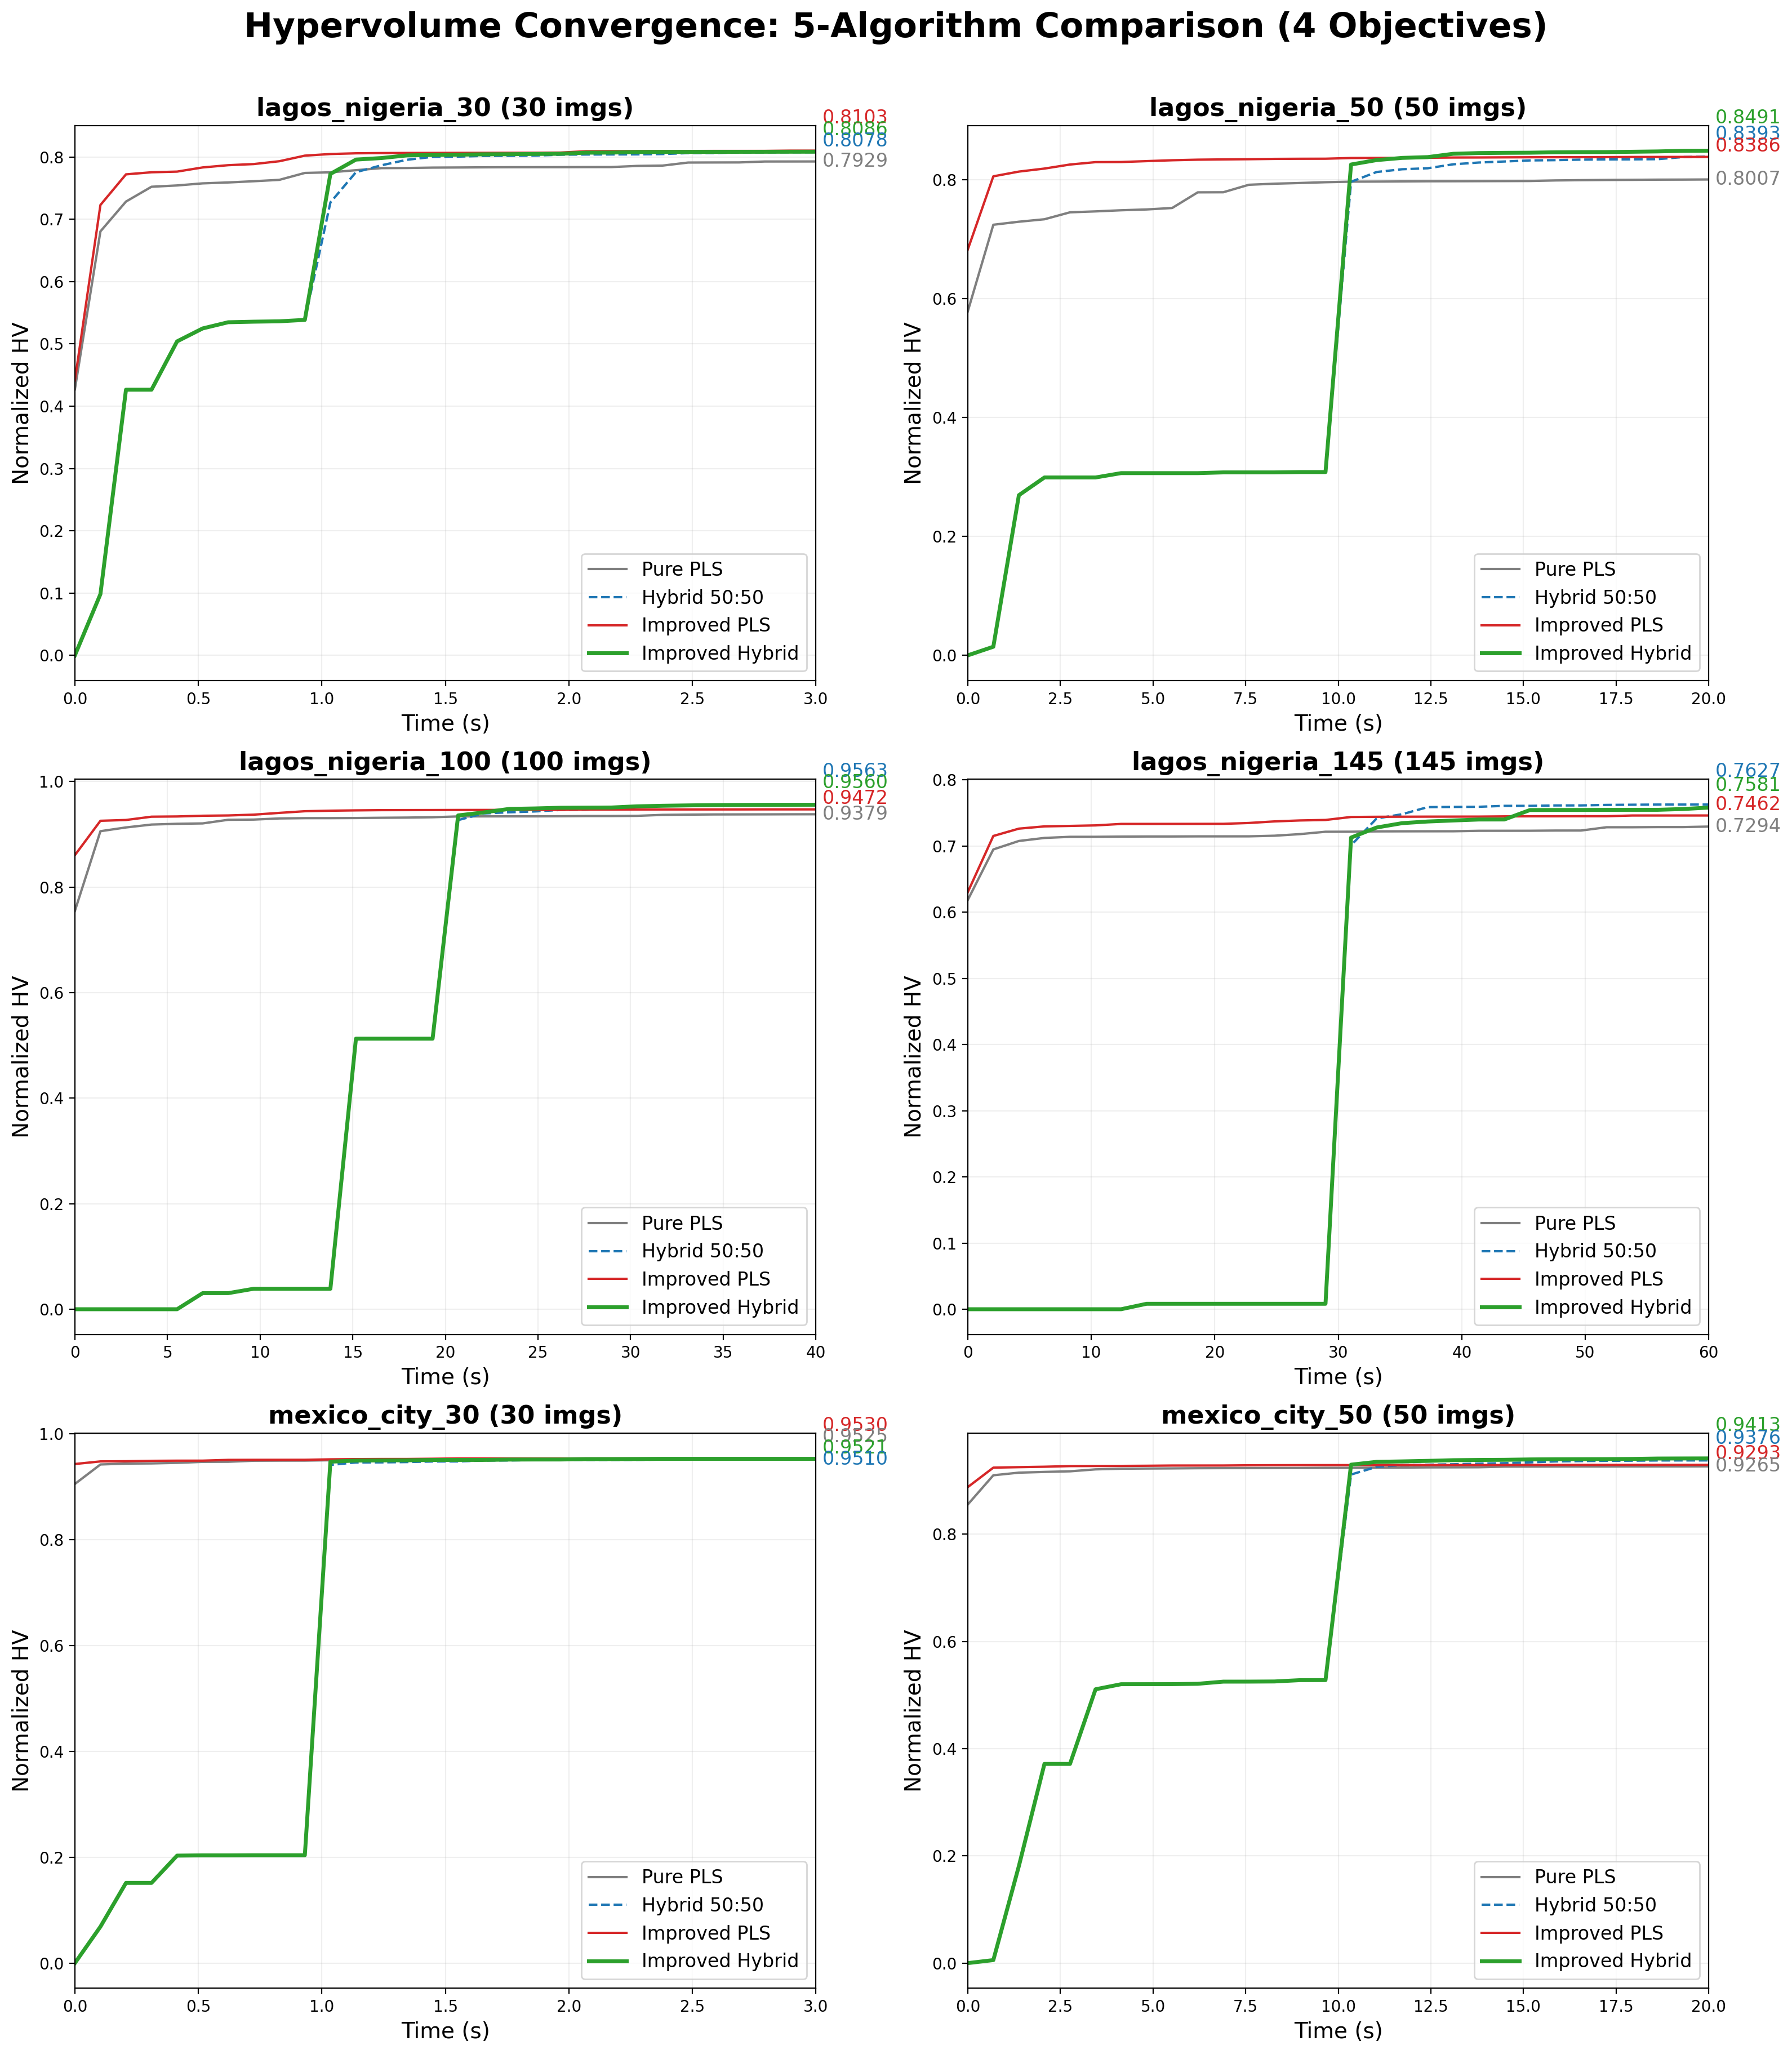
\includegraphics[width=\textwidth]{../../hv_experiment_results/fig_combined.png}
\caption{Normalised hypervolume over time for six representative
  instances (4~objectives).  The {\color{improved}green} curve (enhanced
  PLS) consistently dominates the {\color{baseline}grey} curve (baseline)
  after the first seconds.}\label{fig:hv_curves}
\end{figure}

\subsection{Configuration Comparison}

To isolate the contributions of the PLS enhancements and the hybrid MILP
component, \Cref{tab:ablation} compares all four configurations on the
size-50 and size-100 instances.

\begin{table}[t]
\centering
\caption{Normalised hypervolume for all four configurations on size-50
  and size-100 instances.  Bold indicates improvement $\ge 1\%$ over
  Pure PLS baseline.}\label{tab:ablation}
\small
\begin{tabular}{lrrrr}
\toprule
& \textbf{Hybrid 50:50} & \textbf{Hybrid} &
  \textbf{Imp.\ PLS} & \textbf{Imp.\ Hybrid} \\
\midrule
\multicolumn{5}{l}{\textit{Size 50}} \\
Lagos 50   & 0.801 & \textbf{0.839} & \textbf{0.839} & \textbf{0.849} \\
Mexico 50  & 0.927 & \textbf{0.938} & 0.929 & \textbf{0.941} \\
Paris 50   & 0.857 & 0.864 & 0.858 & 0.864 \\
Rio 50     & 0.655 & 0.654 & 0.657 & \textbf{0.665} \\
Tokyo 50   & 0.909 & 0.917 & 0.911 & 0.918 \\
\midrule
\multicolumn{5}{l}{\textit{Size 100}} \\
Lagos 100   & 0.938 & \textbf{0.956} & 0.947 & \textbf{0.956} \\
Mexico 100  & 0.784 & \textbf{0.821} & \textbf{0.869} & \textbf{0.874} \\
Paris 100   & 0.752 & \textbf{0.874} & \textbf{0.926} & \textbf{0.929} \\
Rio 100     & 0.955 & \textbf{0.974} & 0.959 & \textbf{0.974} \\
Tokyo 100   & 0.919 & 0.920 & 0.922 & 0.923 \\
\bottomrule
\end{tabular}
\end{table}

The comparison reveals complementary strengths:
\begin{itemize}[nosep]
  \item \textbf{Hybrid 50:50} consistently outperforms Pure PLS on
    size-100 instances where exact MILP can produce high-quality seed
    solutions (Lagos, Mexico~City, Paris, Rio).  On size-50 instances
    the gains are more modest since the MILP budget is proportionally
    larger relative to the instance difficulty.
  \item \textbf{Improved PLS} delivers the largest gains on instances
    where the PLS search itself benefits from better initialisation and
    escape mechanisms (Mexico~City~100, Paris~100, Paris~150).  On
    Paris~100 the Improved PLS HV~($0.926$) already surpasses the
    Hybrid~($0.874$), showing that PLS quality can exceed MILP seeding
    on certain instances.
  \item \textbf{Improved Hybrid} matches or exceeds both single-approach
    configurations on every instance, confirming that the two strategies
    are complementary: MILP provides a strong starting front while the
    PLS enhancements maximise subsequent exploration.
  \item \textbf{Size-50 instances} are less discriminating since most
    configurations converge to similar HV values within the 20\,s
    budget; the differences become much more pronounced at 40\,s
    (size-100) and 60\,s (size-150).
\end{itemize}

\subsection{Improvement Summary}

\Cref{fig:bar_summary} provides a visual summary of per-instance HV
improvements.

\begin{figure}[t]
\centering

\includegraphics[height=0.86\textheight,keepaspectratio]{../../hv_experiment_results/fig_barchart.png}
\caption{Per-instance normalised hypervolume improvement of the
  enhanced PLS over the baseline.  Instances are ordered by city and
  size.}\label{fig:bar_summary}
\end{figure}

% ══════════════════════════════════════════════════════════════════════
\section{Discussion}\label{sec:discussion}

\paragraph{Why does greedy initialisation help so much?}
The SIMS objective space is inherently heterogeneous: $f_1$ (cost) and
$f_4$ (angle) are per-image, while $f_2$ (cloud) and $f_3$ (resolution)
are per-element.  A solution minimising cost aggressively selects few,
cheap images; one minimising cloud selects images with maximal clear
coverage; one minimising angle avoids high-angle acquisitions entirely.
These are structurally very different solutions (different image counts,
different spatial coverage patterns), and random construction is
unlikely to produce any of them.  The greedy construction targets each
extreme and the pairwise trade-offs between them, providing the PLS with
well-separated starting points that span the Pareto front.

\paragraph{When does perturbation restart matter?}
Perturbation is most beneficial on instances with \emph{sparse
neighbourhoods}---those where few unselected images overlap with
selected ones, causing the $k{=}1$ neighbourhood to be quickly
exhausted.  This is characteristic of instances with high coverage
redundancy (many images covering the same elements) where good solutions
use few images, leaving few replaceable candidates.  Rio de Janeiro and
Tokyo Bay exhibit this pattern.

\paragraph{Checkpoint overhead.}
The checkpoint mechanism introduces a small memory overhead (two
copies of the mutable tracker state, ${\approx}52$\,KB for 100-image
instances) but provides a consistent speedup of $5$--$15\%$ in
neighbourhood evaluation throughput, which compounds over the entire
run.

\paragraph{Limitations.}
On size-30 instances the enhancements provide negligible improvements
($0.0\%$ to $+2.0\%$), because the baseline already explores the
objective space near-exhaustively within the 3\,s budget.  These small
deltas are within the noise range of single-seed deterministic runs and
would likely vanish with multi-seed averaging.

% ══════════════════════════════════════════════════════════════════════
\section{Related Work}\label{sec:related}

\paragraph{Pareto Local Search.}
PLS was introduced by Paquete et al. and extended
with variable neighbourhood structures by Liefooghe et
al..  Our checkpoint mechanism is, to our
knowledge, the first application of bulk state snapshotting to
incremental objective trackers in PLS.

\paragraph{Initialisation in multi-objective metaheuristics.}
The importance of initial population quality is well established for
evolutionary algorithms.  Decomposition-based
methods (MOEA/D) use weight vectors to structure
the search; our greedy initialisation adapts this idea to PLS by using
weight vectors to construct diverse feasible solutions rather than to
decompose the optimisation.

\paragraph{Perturbation and restart strategies.}
Iterated Local Search uses perturbation to escape
local optima in single-objective settings.  Our perturbation restart
extends this idea to the multi-objective PLS context, where the
perturbation is applied to the entire Pareto archive and the perturbed
solutions must satisfy both feasibility and non-dominance criteria.

\paragraph{Satellite image selection.}
The SIMS problem has been studied with MILP
methods and heuristic
approaches.  Our work focuses on
improving the PLS component of a hybrid exact/heuristic framework.

% ══════════════════════════════════════════════════════════════════════
\section{Conclusion}\label{sec:conclusion}

We presented three complementary enhancements to Pareto Local Search
for the four-objective Satellite Image Mosaic Selection problem:
greedy multi-objective initialisation, two-level checkpoint-based
tracker restoration, and perturbation-based restart.

Experimental evaluation on 20~benchmark instances shows that the
combined enhancements improve normalised hypervolume by $+11.7\%$ on
average for instances with 50 or more images, with individual gains
reaching $+57.8\%$ on the hardest instance.  Ablation analysis confirms
that each technique contributes independently: greedy initialisation
provides the largest single improvement by seeding diverse anchor
solutions; perturbation restart rescues the search on instances with
sparse neighbourhoods; and checkpointing consistently increases
exploration throughput.

All enhancements are implemented as runtime-toggleable flags in the
open-source PLS implementation, enabling reproducible ablation studies
and seamless integration into the hybrid solver framework.

\paragraph{Future work.}
Natural extensions include (i)~adaptive weight-vector generation for
the greedy initialisation based on coverage gaps in the current Pareto
front, (ii)~multi-point perturbations (swap 2--3~images) for stronger
diversification, (iii)~integration with decomposition-based search
directions (MOEA/D-style) within the PLS framework, and
(iv)~evaluation on the 200-image instances where the
computational budget must be managed more aggressively.

% ══════════════════════════════════════════════════════════════════════
\paragraph{Acknowledgements.}
Computational experiments were conducted on a workstation with an AMD
Ryzen processor running Linux.  The implementation uses the Rust
programming language with PyO3 bindings.

% ══════════════════════════════════════════════════════════════════════


\end{document}
